\chapter{Proposed Data Structure for Modular Virtual Commissioning} \label{sec:DataStructure}
    Based on the previous findings, a data structure for a virtual commissioning is presented in this chapter. The main objective of this data structure is a high compatibility and a modular design in order to be able to represent the individual sub-components of a real plant. The data structure itself should contain all necessary information required for a virtual commissioning.
    
\section{Layout of the Data Structure}
    % Die tatsächliche Struktur
    The actual layout of the data structure is kept simple and consists of a root folder with several directories for the relevant information as shown in \autoref{fig:DataStruktureHierachry}. The sub-directories contain the information of kinematization and CAD, physical model, PLC source code and documentation. An optional \textit{ReadMe} file is used for general information and revision control of the structure itself. Finally the root folder is compressed into a \textit{.zip} file for distribution. 
	\begin{figure}[htp]
		\centering
		\footnotesize
        \tikzstyle{every node}=[draw=black,thick,anchor=west]
        \tikzstyle{basis}=[draw=black,fill=black!10]
        \begin{tikzpicture}[%
            grow via three points={one child at (0.5,-0.7) and
            two children at (0.5,-0.7) and (0.5,-1.4)},
            edge from parent path={(\tikzparentnode.south) |- (\tikzchildnode.west)}]
            \node [basis] {Data Structure}
            child { node {ReadMe}}	
            child { node {Geometry and Kinematization (CAD)}}		
            child { node {PLC Source Code}}
            child { node {Physical Model}}
            child { node {Documentation}}
            child { node {\dots}}			
            child [missing] {}				
            child [missing] {}				
            child [missing] {};
        \end{tikzpicture}
		\caption[Layout of proposed data structure.]{Layout of proposed data structure. The structure consists of a \textit{ReadMe} file with general information of the structure itself and several folders with the needed information of a virtual commissioning.}
		\label{fig:DataStruktureHierachry}
	\end{figure}

    % Modularität
    Due to the plain and simple structure, it can be easily extended and modular exchanged. In order to show this characteristic, an example of a filling stations as part of a larger plant is considered. The design of this station is shown in \autoref{fig:DataStruktureUseLayout} and consists of a separation (A), two identical dosing units (B) and a conveyor belt (C). These sub-components are bought-in parts and are assembled in this station. The product for the customer is the filling station as a complete unit.  \\
    
    The starting point for the development of the filling station are the exchange packages of the three suppliers with the respective product as content. These packages are connected and expanded and finally result in a package with the entire filling station as seen by the customer. In a next step, the customer can use the filling station represented in just one data structure in planning of the remaining plant. This general procedure is shown in \autoref{fig:DataStruktureComponents}.
	\begin{figure}[htp]
		\centering
		\begin{subfigure}{.30\textwidth}
			\centering
			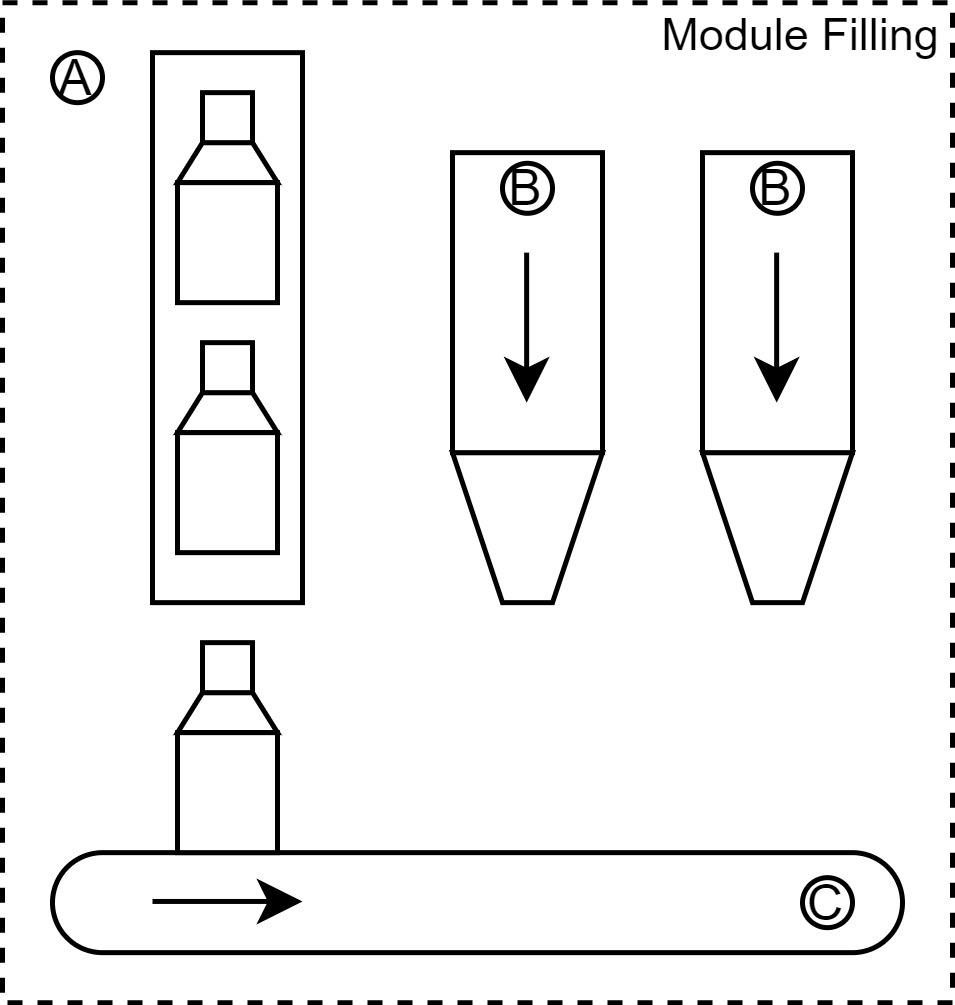
\includegraphics[width=.95\linewidth]{figures/UseCaseDataStructureOverviewProduct.jpg}
			\caption{Product overview}
			\label{fig:DataStruktureUseLayout}
		\end{subfigure}
		\hspace{20mm}
		\begin{subfigure}{.45\textwidth}
			\centering
		%	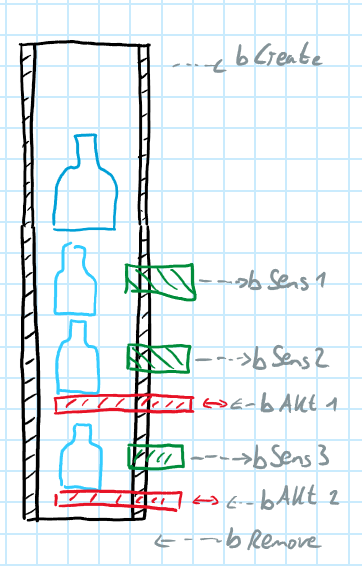
\includegraphics[width=.9\linewidth]{figures/VereinzelungIOs.PNG}
		    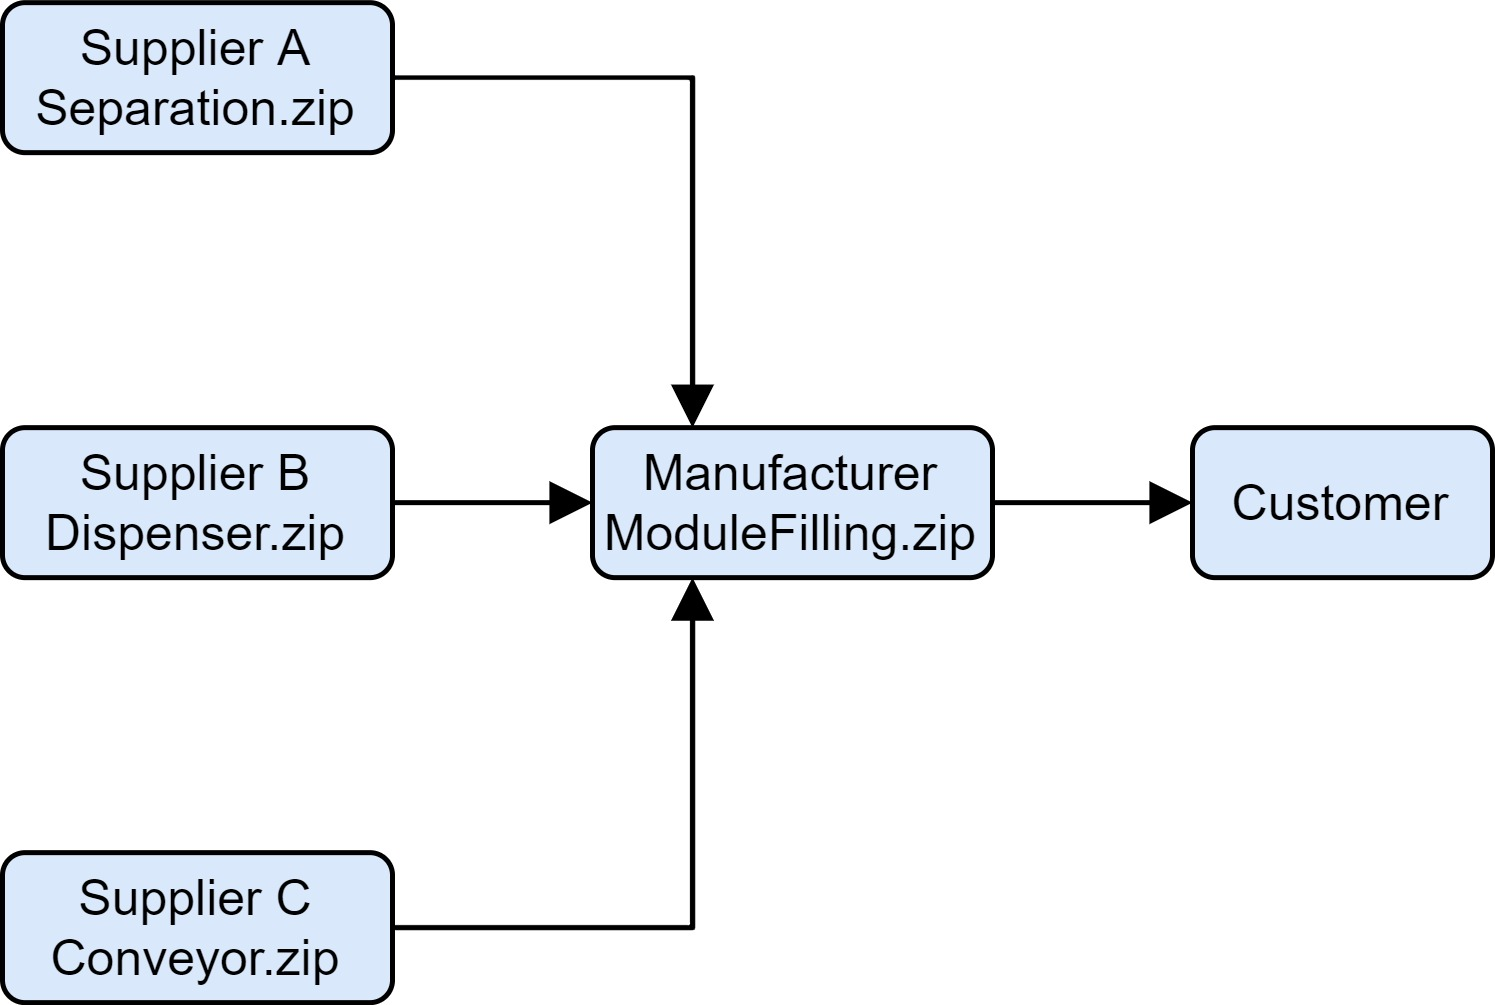
\includegraphics[width=.95\linewidth]{figures/UseCaseDataStructureFileComponents.jpg}
			\caption{File components}
			\label{fig:DataStruktureComponents}
		\end{subfigure}
		\caption[Use case to show modularity of a data structure.]{Use case to show modularity of a data structure. In this case a filling station is considered consisting of a separation (A), dosing units (B) and a conveyor belt (C). The components are bought and merged into a single module.}
		\label{fig:DataStruktureUseCase}
	\end{figure}

    
    
\section{Methods for the Selection of Data Formats}
    In this section, different methods for the virtual commissioning of a simple component are investigated. For this purpose, the different aspects CAD, physical behaviour model and PLC source code are considered and the suitability of different approaches are evaluated. Based on these results, the selection of data formats in the proposed data structure is afterwards made. The used software for this investigation is listed in \autoref{tab:UsedSoftwareForSelectionFormats}.\\
      \begin{table}[htp]
    	\footnotesize
    	\centering
    	\caption{Used software for selection of data formats.}
    	\begin{tabular}{ll}
    		\toprule
    		\multicolumn{1}{c}{Area} & \multicolumn{1}{c}{Used Software}  \\
    		\midrule
    		CAD & Autodesk Inventor Professional 2022\\
    		    & Autodesk 3ds Max 2022 \\
    		    & \\
		    PLC & Beckhoff TwinCAT 3 Version 3.1.4024.25\\
		      & \\
	        Modelling  & Matlab R2020b, Simulink\\
    		\bottomrule
    	\end{tabular}	
    	\label{tab:UsedSoftwareForSelectionFormats}
    \end{table}
    
    The assembly from \autoref{fig:ApproachesGeometryExample} is used as an example for a real plant. Here, a PLC is controlling the speed of the disk in the left section and thus the position of the piston in the right section. The CAD assembly is kinematized and the model of the system describes the angular position of the disc and the position of the piston as a function of the current velocity.
  
    
\subsection{Geometry Data and Kinematization}
    When selecting a suitable format for the CAD data, the support of the kinematics is the main focus. For this purpose, an example assembly of a movable piston is created, as shown in \autoref{fig:ApproachesGeometryExample}. The kinematization consists of a rotating motion of the disk in the left section and a translational motion of the piston in the right section. These two parts are connect by a connecting rod in the middle area, with a rotational axis in both cases. If the left disk rotates, the rotational movement is then transformed into a translational movement of the right piston.\\
	\begin{figure}[ht]
		\centering
		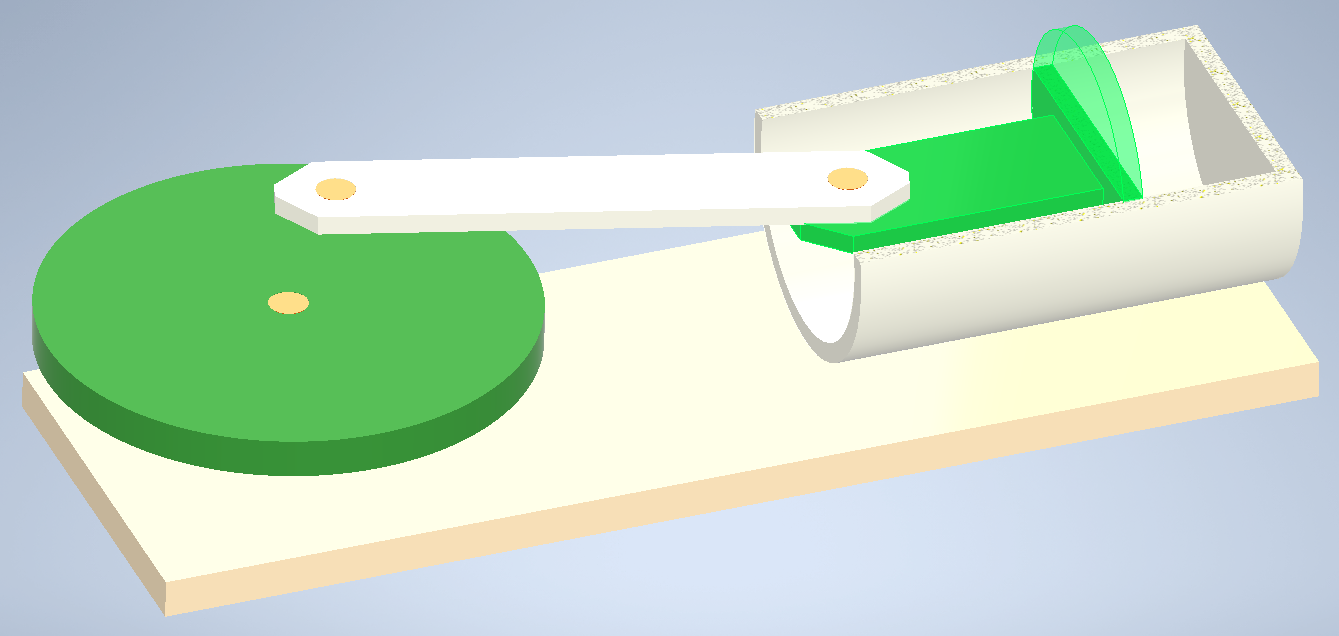
\includegraphics[width=.6\linewidth]{figures/ApproachCadAssembly.PNG}
		\caption[Exemplary assembly for selection of suitable CAD formats.]{Exemplary assembly for selection of suitable CAD formats. For this a movable piston is considered as a plant. The position of this piston is controlled using the disk on the left side.}
		\label{fig:ApproachesGeometryExample}
	\end{figure}
    
    The selection criterion for a suitable exchange format is the ability to save the geometry and kinematization of an assembly in combination with a high compatibility with different tools. As a result of these criteria, a neutral exchange format should provide an optimal solution.  \\
    However, due to the fact that no default exchange format for kinematization exist, different approaches have to be tested. For this purpose, different methods of CAD data exchange are investigated and described in the following sections. An overview of the tested methods is provided in \autoref{fig:ApproachesGeometryOverview}.\\
	\begin{figure}[ht]
		\centering
%		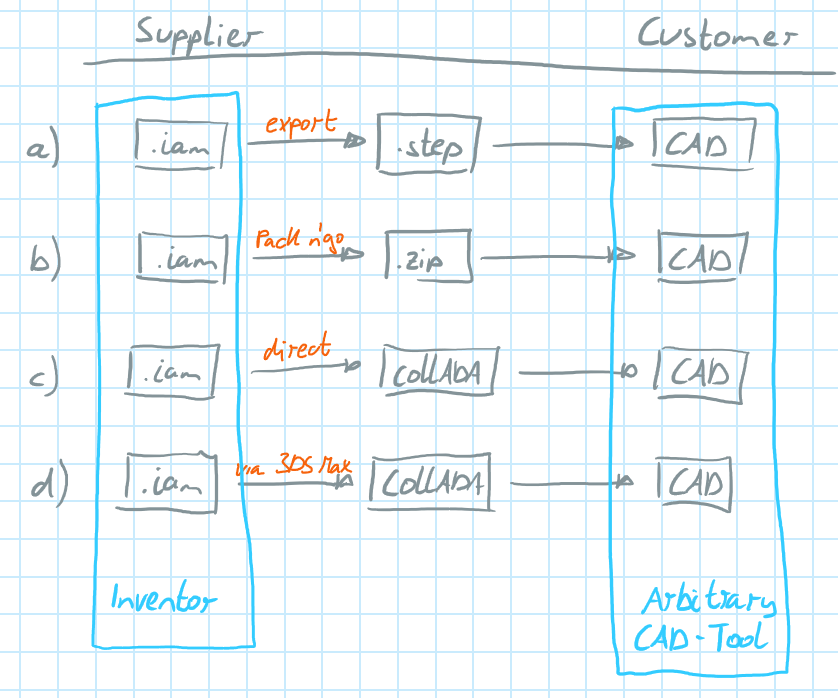
\includegraphics[width=.5\linewidth]{figures/MethodsCadOverview.PNG}
		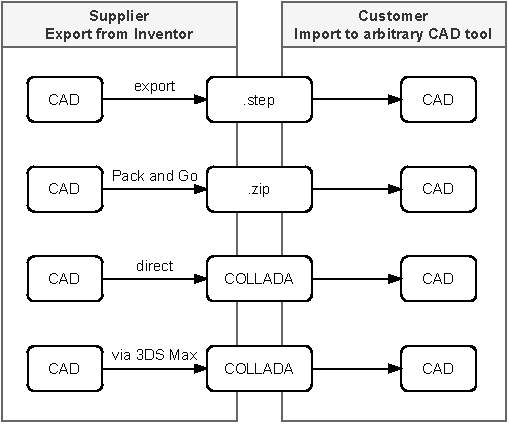
\includegraphics{figures/MethodsOverviewCAD.pdf}
		\caption[Overview of approaches for exchange of geometry with kinematization.] {Overview of tested approaches for exchange of geometry with kinematization. In total four approaches are tested, with the neutral \textit{.step} format, the native \textit{Pack and Go} tool and the neutral \textit{COLLADA} format being investigated. }
		\label{fig:ApproachesGeometryOverview}
	\end{figure}

    
    
\subsubsection{a) \textit{Inventor} to \textit{.step} and back}
    The first approach is using the \textit{.step} format. This neutral format is chosen because it is already widely used for CAD data exchange. \\
    The export of the assembly into a \textit{.step} file is done according to the instruction \cite{InventorAnleitungExportStep} via the menu \textit{File}-\textit{Export}-\textit{CAD Format}. In the appearing window, the target format must finally be set to \textit{.step}. Additional options are not needed. \\
    The import is also very simple and can be done either in a new file or in an existing assembly, where instructions can be found in \cite{InventorAnleitungImportStep}. In this case the \textit{.step} file is opened in a new file via \textit{File}-\textit{Open}. \\
    Exporting and importing \textit{.step} files works without any problems, but the missing kinematic is detected when inspecting the imported assembly. However, the pure geometry is imported without errors and even the hierarchy of parts is created by an integrated conversion during import. In any case, the desired criteria are not met and thus this approach does not represent an optimal solution.
    
\subsubsection{b) \textit{Inventor} to \textit{Pack and Go} and back}
    In the next attempt, the export and import using the \textit{Pack and Go} tool will be investigated in more detail. Here, the entire assembly is bundled into one \textit{.zip} file, allowing an easier handling in the distribution of the final data. \\
    The export of the assembly into a bundled \textit{.zip} file is done according to the instruction \cite{InventorAnleitungExportPackAndGo} via \textit{File}-\textit{Save as}-\textit{Pack and Go}. Here, in addition to the individual components, related project data is also exported.   \\
    For import this \textit{.zip}-file only has to be extracted and afterwards can be opened via \textit{File}-\textit{Open}. In this case the main assembly of the project can be opend afterwards and no information is lost.  \\
    Because of this simple handling, exporting and importing is done in a short time and without losing any information between two instances of \textit{Inventor}. However, by keeping the native file formats, the high compatibility to other CAD software is missing and as a result this way is also not an ideal solution for open data exchange. 
    
\subsubsection{c) \textit{Inventor} to \textit{COLLADA} and back}
    Direct export and import of \textit{COLLADA} files is currently not officially supported by \textit{Inventor}. Freely available but also commercial 3rd party tools partly offer a possibility to export CAD data. An example of a commercial solution for exporting from \textit{Inventor} to \textit{COLLADA} is shown by \cite{ColladaExportPlugin} in form of a \textit{Inventor} plugin. Importing \textit{COLLADA} back into the native formats of \textit{Inventor} is still a challenge, which can only be solved with great effort. In this case, in practice, often the recreation of the \textit{COLLADA} data in \textit{Inventor} is a faster solution compared to the time-consuming import. A problem of the 3rd party software is the mostly missing implementation of new versions of \textit{COLLADA} resulting in the missing support of the kinematization during the export.  
    
\subsubsection{d) \textit{Inventor} to \textit{3DS Max} to \textit{COLLADA} and back}
    CAD data from \textit{Inventor} can also be exported to the desired \textit{COLLADA} format via an intermediate step using the software \textit{3DS Max}. The advantage of this compared to the previous approach is the native tool chain of \textit{Autodesk} with the avoidance of 3rd party tools, but with the limitation of an export of the pure geometry. However, the problem remains similar with feasible support for export, but lack of possibilities for import of \textit{COLLADA} files. \\
    For example, opening \textit{Inventor} files in \textit{3DS Max} is done using the guide \cite{DsMaxAnleitungImportInventor}. Further, a \textit{COLLADA} file can be then exported using \textit{File}-\textit{Export}-\textit{Export}. \\ 
    In the same way, importing a \textit{COLLADA} into \textit{3DS Max} is done via \textit{File}-\textit{Import}-\textit{Import} without any major difficulties. However, the next step, consisting of exporting to an \textit{Inventor} file from \textit{3DS Max}, is not supported. For this reason, this method is also not a satisfying solution.
    
\subsection{Behaviour Model}    \label{sec:MethodsModel}
    Since the \textit{FMI} format is supported by a large number of tools, it has already been established as the unofficial standard format for data exchange of models in the industry. For this reason, no other data format for describing behaviour models will be further investigated in this thesis. \\
    
    What is tested, however, is the practical use by means of an example with the given software. For this purpose a model of the moving piston is created in \textit{Simulink} and is afterwards exported to the \textit{FMI} format. The final goal of this evaluation is the integration of this model into the PLC run-time. \\
    The model describes the position of the piston and the angle of the disk depending on the velocity of the disk. The rotation speed of the disc is the output of the control on the PLC, where the position of the piston should be controlled. This model in \textit{Simulink} is shown in \autoref{fig:ApproachesModel}. 
	\begin{figure}[htp]
		\centering
		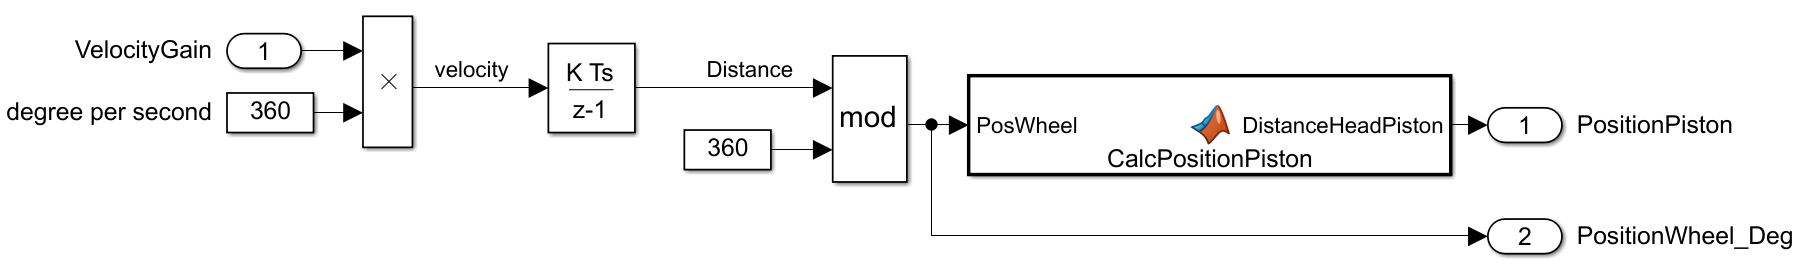
\includegraphics[width=.99\linewidth]{figures/ApproachModelInSimulink.PNG}
		\caption{Example for testing the behaviour model.} 
		\label{fig:ApproachesModel}
	\end{figure}
	
    An overview of the methods to integrate the model in the PLC can be found in \autoref{fig:ApproachesModellingOverview}.
	\begin{figure}[htp]
		\centering
%		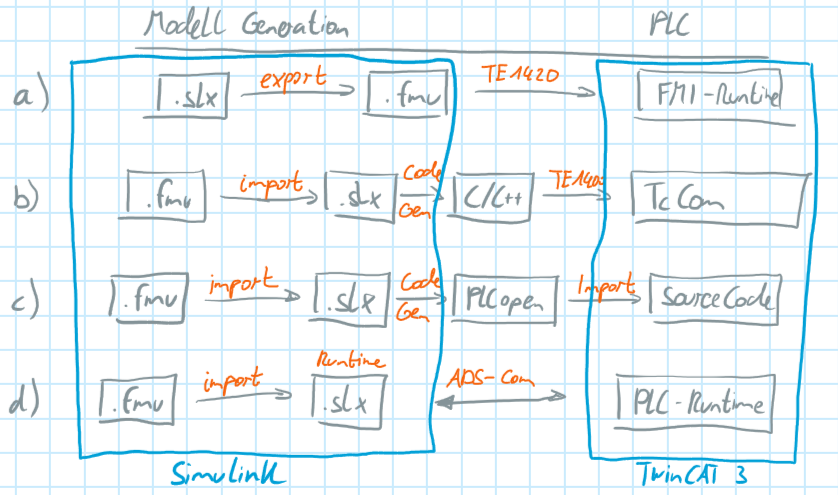
\includegraphics[width=.7\linewidth]{figures/ApproachModelOverview.PNG}
		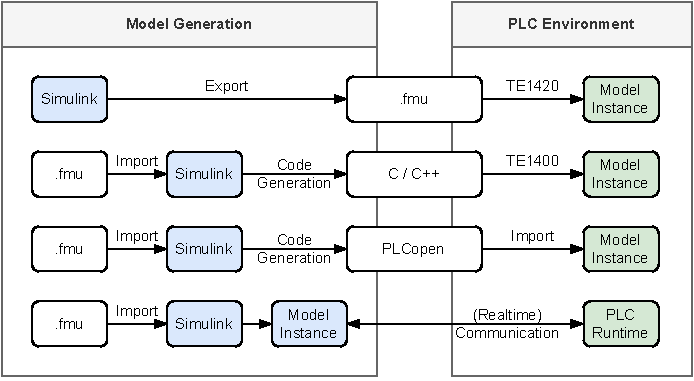
\includegraphics{figures/MethodsOverviewModel.pdf}
		\caption[Overview of tested methods for \textit{FMI} handling.] {Overview of tested methods for \textit{FMI} handling. In total four approaches are tested in order to use a \textit{.fmu} model in a PLC run time. The blue blocks are required steps in \textit{Simulink} and the green ones are located in the \textit{PLC}.} 
		\label{fig:ApproachesModellingOverview}
	\end{figure}
	
    
    
    
\subsubsection{a) Run \textit{FMI}-Unit directly in \textit{TwinCAT}}
    The first approach is also in this case the direct use of the \textit{FMI} object in \textit{TwinCAT}. This offers the advantage that the model can be executed directly on the PLC and thus a real-time capability is given without any additional steps. Furthermore, possible restrictions and problems can be avoided when using 3rd party tools. In order to integrate the \textit{FMI} model, \textit{Beckhoff} offers the product \textit{TE1420} containing the \textit{FMI} interface to the run-time of a PLC \cite{BeckhoffFmiProduct}. With this interface it should be possible to create an object for \textit{TwinCAT} directly from the \textit{FMI} file. This object would then have the defined inputs and outputs and could be integrated and linked in the software of the PLC. This would allow to directly use the current values of the behaviour model in the software of the PLC. \\ 
    
    Since this interface is still under development at the time of writing this thesis, alternative approaches for integrating an \textit{FMI} file in a virtual commissioning have to be found. This method is currently rejected due to the missing interface, but should be investigated again in the near future. 
    
\subsubsection{b) \textit{FMI} import in \textit{Simulink} and export to \textit{TwinCAT}}
    In this approach the target for \textit{Simulink} of \textit{TwinCAT} is analyzed. This target is part of the product \textit{TE1400} and allows the integration of \textit{Simulink} models into \textit{TwinCAT} by using the \textit{Simulink Coder}. In this process, C/C++ code is generated from the model in the first step and further transformed into a \textit{TcCom} object in \textit{TwinCAT}. When using the free trial version of \textit{TE1400}, attention must be paid to the limitation of a maximum of five input and five output variables \cite{TwincatManualTE1400}. However, this limitation does not apply to the commercial version. \\
    
    The integration of the model in \textit{TwinCAT} using this method is done similar to the example \textit{SimpleTemperatureControl} from the documentation of the product \textit{TE1400}. \cite{TwincatTcComSamples}. \\
    For this, the \textit{System target file} must be set to \textit{TwinCatGrt.tlc} in the code generation settings. The remaining settings of the code generation can be kept, but the solver must be set to the type \textit{fixed-step} with the step size equal to the task time of the PLC. After successful code generation the \textit{TcCom} object must be signed as described in the instructions. Afterwards it can be included and used in \textit{TwinCAT}.\\
    In this evaluation, first the original model of \textit{Simulink} is exported and then in the same way the \textit{FMI} object.\\
  %  In the same way, the model with the \textit{FMI} object is processed. However, code generation fails due to missing support of the \textit{FMI} block in the part of \textit{code generation} of \textit{Simulink}. \\
    
    The export of the original \textit{Simulink} model works without problems and a \textit{TwinCAT} object can be created. In the same way, the model with the \textit{FMI} object is processed, but In contrast the export of the object fails, due to missing support of the special \textit{FMI} block in the code generation of \textit{Simulink}. As a result, this method is not a suitable solution for the given software in virtual commissioning. However, if a supported model is available in \textit{Simulink} the code generation can be a useful way to include it in \textit{TwinCAT}.  
    
    

\subsubsection{c) \textit{FMI} import in \textit{Simulink} and export to \textit{PLCopen}}
    Similar to the previous approach, the code generation of \textit{Simulink} is further investigated here, but with the difference of the target platform. While in the previous approach C/C++ code was generated from the original model, here it will be exported directly to the \textit{PLCopen} format. This can be then easily integrated and used in \textit{TwinCAT} in the next step.\\
    
    The export to \textit{PLCopen} format via \textit{Simulink PLC Coder} is done analog to the example \textit{Generate Structured Text Code for a Simple Simulink Subsystem} \cite{SimulinkPlcCoderExample} also first for the original model and then for the model with the \textit{FMI} object. When using the PLC coder, attention must be paid to the supported blocks used in the model. For example, continuous blocks can only be used in some cases and must therefore be replaced by discrete alternatives. An example of this is a continuous transfer function which is not supported and must therefore first be discretized. \\
    
    The used time-discrete model can be exported without major issues similar to the method before. Additional settings besides the \textit{fixed-step} solver are not necessary and the model can now be included and used as \textit{function block} in \textit{TwinCAT}. \\
    As already suspected, the export of the model with the \textit{FMI} object is not possible. As before, the \textit{FMI} block is not supported in the code generation of the \textit{Simulink PLC Coder}, which can also be seen in the list of supported blocks \cite{SimulinkPlcCoderSupportedBlocks}. Like the previous approach, this solution is also rejected for this reason. 
    
\subsubsection{d) \textit{FMI} import in \textit{Simulink} and communication with \textit{TwinCAT}}
    This approach differs from the previous ones by the target of the model run-time. Compared to the other approaches, it is not located directly on the PLC, but remains in \textit{Simulink} on the engineering system. However, this also results in additional communication between the PLC and the used engineering system. For time-critical applications, real-time capability for this engineering system is also recommended by means of using special hardware and software. \\
    
    In this case the communication to the PLC is done via the \textit{ADS} interface of \textit{Beckhoff}. This communication is integrated via special blocks in \textit{Simulink} and is here done via the block \textit{TwinCAT Symbol Interface} \cite{TwincatAdsBlocks}. These blocks are part of the product \textit{TE1410} which contains the interface to Simulink and also in this product the limitation of the number of variables in the test version has to be considered \cite{TwincatManualTE1410}. \\
    After the configuration of the \textit{interface} block the PLC variables are available as source/sink in \textit{Simulink} and can be connected to the model. The solver must also be set to \textit{fixed-step} again with the same step size as the task time of the PLC. \\
    With this method the model can be used in its original form and exported as \textit{FMI} object. Thus inputs can be read from the PLC and outputs can be written. In other words, this method is not an ideal or simple solution, but it provides a feasible way to integrate \textit{FMI} objects into \textit{TwinCAT} and thus perform a virtual commissioning.  

\subsection{PLC Code}
    The \textit{PLCopen} format already represents a standardized interface for the exchange of PLC code, since the format is well established in the industry and defined by an international standard. For this reason, the review of alternative formats for data exchange can be skipped and only the implementation of the \textit{PLCopen} format in \textit{TwinCAT} needs to be examined.  \\
    
    The export and import is tested using again the moving piston. The aim of the PLC is to set the velocity of the disc in order to control the position of the piston. This is done by defining a variable for the speed and a variable for the position of the piston. Additionally, a variable for the angular position of the disk is defined, which can be used in a visualization. Depending on the set velocity, the program then calculates the position of the piston. The source code is listed in the \textit{PLCopen} format in \autoref{lst:ApproachExampleCode}. 
    \lstinputlisting[basicstyle=\tiny, caption={Example Piston as \textit{PLCopen}-xml}, label=lst:ApproachExampleCode]{sourcecode/ApproachTestingPLC.xml}
    
\subsubsection*{\textit{TwinCAT 3} to \textit{PLCopen}}
    The export and import of \textit{PLCopen} objects is supported in \textit{TwinCAT} and is done without difficulty, whereby instructions for this can be found in \cite{TwincatExportPlcopen}. Therefore, using the \textit{PLCopen} format is a suitable solution for data exchange in this case. 



\section{Selected File Formats}
    As already mentioned in \autoref{sec:AvailableDataFormats}, a wide range of possible data formats exists to represent the required information for virtual commissioning. The focus in the selection of the used formats, should be on the widest possible support in different tools. Only through this approach the format can become accepted in the industry. In this section, the selection of suitable data formats is done.
   
    
    % Beschreibung und Begründung für alle Punkte
    \subsection{Geometry Data and Kinematization}
    For a loss-free exchange of CAD data, the information of the kinematization of the assemblies must be preserved in addition to the raw geometry. As mentioned earlier, this is a big problem in practical use and therefore the \textit{COLLADA} format would be an ideal solution. At the moment, suitable tools for conversion are missing or do not support the current version of \textit{COLLADA} implementing the kinematization. As a result, using the \textit{COLLADA} format is the optimal solution in theory but in practice native CAD formats are the better choice if the kinematization should be preserved. Which CAD tool and further which format is finally used has to be defined between the customer and supplier. Alternatively, neutral formats like \textit{.step} can be used, but with the disadvantage of missing kinematics. For these reasons, although a solution exists for the exchange of CAD data, it is not sufficient in the field of virtual commissioning. \\
    
    For example, \textit{Inventor} offers a quick way to exchange data via the \textit{Pack and Go} tool \cite{InventorPackAndGo}. In this case, the entire geometry, dependencies and also materials of an assembly are bundled in one \textit{.zip} file, which also simplifies the exchange. A similar function is also available in \textit{Solidworks} \cite{SolidworksPackAndGo}. It should be noted, that although the two functions have the same name, they are not compatible with each other. \\
    
    An overview of the evaluation of the different approaches can be found in \autoref{tab:ResultsGeometry}.
      \begin{table}[htp]
    	\footnotesize
    	\centering
    	\caption[Results of tested methods in CAD exchange.]{Results of tested methods in CAD exchange evaluated for their usability from bad (\fullmoon  \fullmoon  \fullmoon) to good (\newmoon \newmoon \newmoon). This table shows the characteristics of the tested methods with respect to save geometry in a CAD file, kinematization of an assembly, a wide support for different tools and an overall evaluation of the usability for a virtual commissioning.}
    	\begin{tabular}{lcccc}
    		\toprule
    		\multicolumn{1}{c}{Method} & \multicolumn{1}{c}{Geometry} & \multicolumn{1}{c}{Kinematization} & \multicolumn{1}{c}{wide software support} & \multicolumn{1}{c}{Usability}\\
    		\midrule
    		a) Using \textit{.step} & yes & no & yes & \newmoon \newmoon \fullmoon\\
    		b) Using native \textit{Pack and Go} & yes & yes & no & \newmoon \newmoon \fullmoon\\
    		c) Using \textit{COLLADA} directly & - & - & - & \fullmoon \fullmoon \fullmoon \\
    		d) Using \textit{COLLADA} indirectly & yes & no & no & \newmoon \fullmoon \fullmoon\\
    		\bottomrule
    	\end{tabular}	
    	\label{tab:ResultsGeometry}
    \end{table}
    
    \subsection{Behaviour Model}
    The modeling of the physical behaviour can also be done using various tools. In contrast to CAD data, a neutral and established format for data exchange already exists here: the \textit{FMI}. A growing number of tools support this format, making it a good choice in a modular virtual commissioning process. \\
    
    In the academic community, but also in industry, \textit{Simulink} is often used for modelling. This tool is very popular mainly because of its flexibility, and supports the import and export of \textit{FMI} files in versions 1 and 2. Instructions for the export can be found in \cite{MatlabFmuExport} and for the import in \cite{MatlabFmuImport}. 
    
    The summary of the evaluation of the tested approached can be found in \autoref{tab:ResultsModel}.
    \begin{table}[htp]
    	\footnotesize
    	\centering
    	\caption[Results of tested methods in integrating behaviour model.]{Results of tested methods in integrating behaviour model evaluated for their usability from bad (\fullmoon  \fullmoon  \fullmoon) to good (\newmoon \newmoon \newmoon). This table shows the results of different approaches to include the model from \textit{Simulink} or as \textit{FMI} file in \textit{TwinCAT} and afterwards using it in a virtual commissioning. The evaluation is based on the feasibility of the approaches.}
        \begin{tabular}{lcccc}
            \toprule
            \multicolumn{1}{c}{Method} & \multicolumn{1}{c}{\begin{tabular}[c]{@{}c@{}}Working with \\ \textit{Simulink} model\end{tabular}} & \multicolumn{1}{c}{\begin{tabular}[c]{@{}c@{}}Working with \\ \textit{FMI} model\end{tabular}} & \multicolumn{1}{c}{Real time} & \multicolumn{1}{c}{Usability}\\
            \midrule
            a) Model directly in \textit{TwinCAT} & - & (yes) & (yes) & (\newmoon \newmoon \newmoon)\\
            b) Model to \textit{TcCom}-Object & yes & no & yes & \newmoon \fullmoon \fullmoon \\
            c) Model to \textit{PLCopen} & yes & no & yes & \newmoon \fullmoon \fullmoon \\
            d) Run Model in \textit{Simulink} & yes & yes & no & \newmoon \newmoon \fullmoon \\
            \bottomrule
        \end{tabular}
    	\label{tab:ResultsModel}
    \end{table}
    
    % PLC Code
    \subsection{PLC Code}
    The exchange of PLC code is almost no problem in practice. This is thanks to the standardization of automation engineering using PLCs, which also describes the possible programming languages and the exchange format as \textit{.xml} files. In addition to the language basis, more complex functions such as function blocks for movements are also part of the standard and thus easily exchangeable. Thanks to the international validity, many manufacturers rely on this standardization and offer converters to and from the \textit{PLCopen} format.
    
        % Documentation and Drawings
    \subsection{Documentation}
    For the exchange of documentation, the \textit{.pdf} format has already been proven in practice. One of the reasons for this is the exact same layout of the document regardless of the operating system or a printout on paper. This ensures that the document is available to the reader in exactly the same form as it was when it was created. 
    
    \subsection{Overview of Selected Data Formats}
    An overview of the selected data formats is found in \autoref{tab:InformationAndFormats}.
    \begin{table}[htp]
        \footnotesize
        \centering
        \caption{Chosen file formats for the proposed data structure.}
        \begin{tabular}{lll}
        	\toprule
        	\multicolumn{1}{c}{Discipline} & \multicolumn{1}{c}{Information} & \multicolumn{1}{c}{Choosen File Format}\\
        	\midrule
        	
            Mech. Engineering & CAD (pure geometry) & Neutral formats like \textit{.step}\\
            & CAD (with kinematics) & Native formats like \textit{.iam} or \textit{COLLADA}  \\
            
            & Physical Behavior & \textit{FMI} as \textit{.fmu} \\
            & & \\
            Elec. Engineering & PLC layout  & Native formats or \textit{.pdf} \\
            & List of used inputs and outputs  & Native formats or \textit{.pdf} \\
            & & \\
            Coding & PLC Code & \textit{PLCopen} as \textit{.xml}\\
            & & \\
            General & Documentation & \textit{.pdf}\\
    %         & Drawings & \textit{.pdf}\\
        	\bottomrule	
        \end{tabular}	
        \label{tab:InformationAndFormats}
    \end{table}


\section{Workflow of the Proposed Data Structure} 
    The workflow when using the proposed data structure consists of two main parts: generating the data (export) and using the data in a virtual commissioning (import). The export and import respectively consist of the subcategories of the CAD data, the behaviour model and the control code. The whole workflow is shown in the overview in \autoref{fig:GeneralWorkflow}.\\

    % Beschreibung Export
    Compared to the import, the export of the data is more straightforward and thus easier to accomplish. The data can usually be generated in just a few steps, with CAD data being the exception to this general rule. In principle, the greatest effort is required when using the data structure in the field of CAD data, due to the lack of an interface for saving the kinematics of an assembly. If only the geometry should or can be transferred, a neutral format like \textit{.step} or \textit{.iges} is recommended, which are supported by most of the CAD tools. Until the \textit{COLLADA} format or alternatives are established in industry, exporting kinematics is done easiest in native CAD formats. The choice of the used software should be made in a close cooperation between the supplier and the customer and thus depends on the specific application. \\
    In comparison, the export of the behaviour model, the control code of the PLC and, if necessary, a technical documentation do not cause major problems and are supported by the majority of available software.\\
    
    % Beschreibung Import
    The process of importing the data, in contrast to exporting, is more complex, where the individual steps strongly depend on the used target software. In the case of CAD data, it is necessary to distinguish between three possible approaches: the assembly is not kinematized (for example \textit{.step}), the assembly is kinematized in neutral format (for example \textit{COLLADA}) and the assembly is kinematized in a native format (for example \textit{.iam}). The native format provides the least effort for integration, followed by plain geometry without kinematization (depending on the complexity of the assembly). The greatest effort represents the import of a \textit{COLLADA} file, due to the lack of conversion tools. \\
    %After importing the geometry and recreating the kinematization if needed, communication with the PLC must be established. The goal of this communication is to visualize the current status of the PLC. For this purpose, the plug-in functionality of the various CAD software in combination with existing interfaces of the PLC often provides a suitable solution. \\
    The import of the PLC code is done in the majority of PLC systems without any difficulties thanks to the international standardization of the programming language. As a result sample code can be integrated into an existing project fast and without any difficulties. \\
    However, with the behaviour model, a dependency to the used software is once again recognizable. In the best case, the \textit{FMI} object can already be executed directly in the PLC and linked to the inputs and outputs of the hardware. Alternatively, the model can be executed in software for simulations, which again communicates with the PLC. If virtual commissioning is performed using this method, special hardware must often be used to ensure real-time capability. However, this requirement only applies to time-critical processes.
	\begin{figure}[ht]
		\centering
%		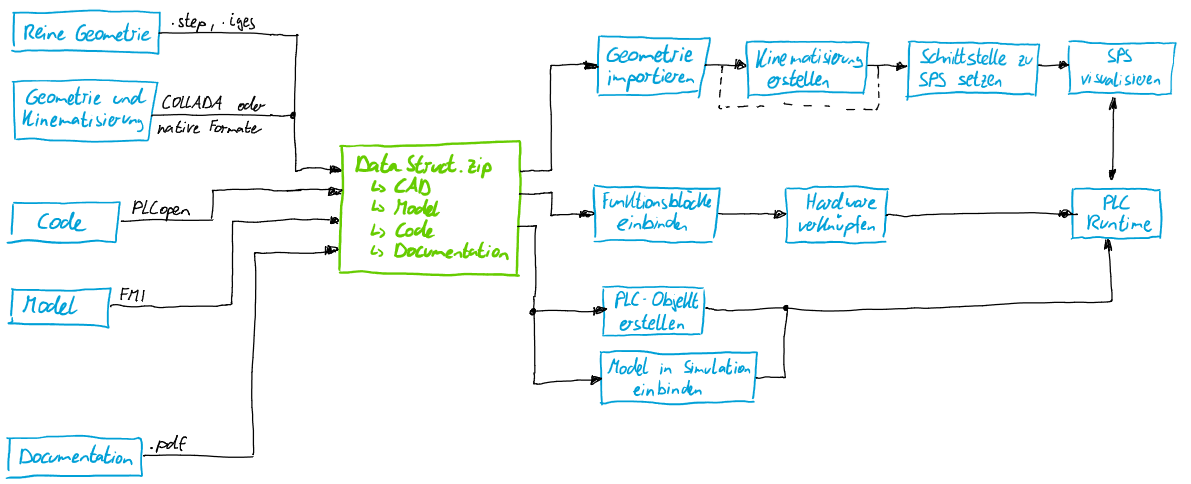
\includegraphics[width=.95\linewidth]{figures/GeneralWorkflow.png}
		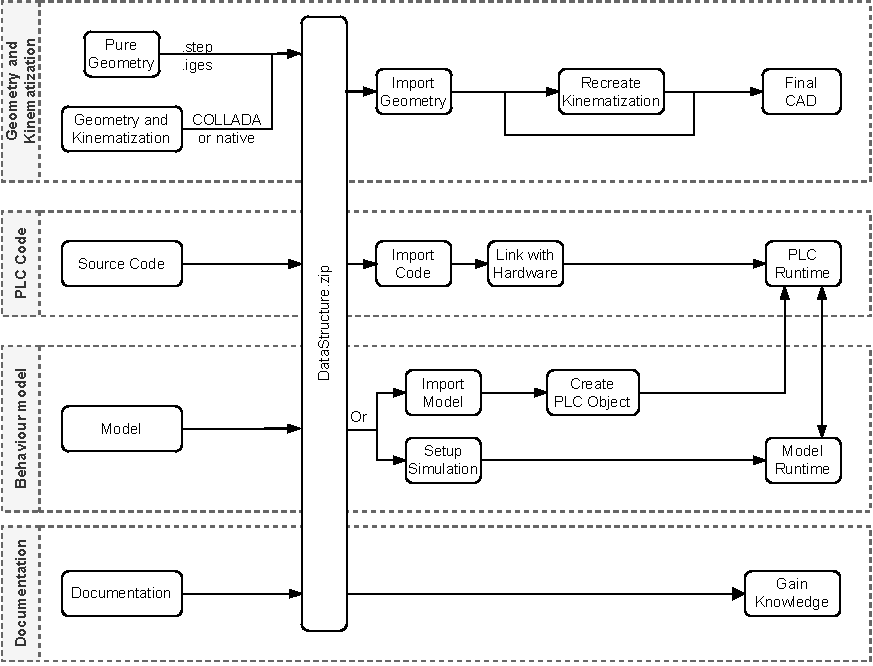
\includegraphics{figures/GeneralWorkflow.pdf}
		\caption[General workflow of proposed data structure.]{General workflow of proposed data structure. In this picture the most important aspects for the export and import of the data structure are shown and divided into the corresponding categories. }
		\label{fig:GeneralWorkflow}
	\end{figure}

	
    
    
\section{Summary}
    This chapter describes the layout and use of a modular data structure. The field of application includes the data exchange for virtual commissioning, where the control is done via a PLC. \\
    The foundation of this structure is a single root folder containing the CAD data (native format or \textit{COLLADA}), the behaviour model (\textit{FMI}), the control software (\textit{PLCopen}) and the associated documentation (\textit{.pdf}). Compressing this structure into a \textit{.zip} file simplifies even more the distribution and sharing.
    In the case of CAD data, no optimal solution has been found yet for the selection of data formats, since kinematization is currently only supported with major problems. However, various approaches to solve this problem are in development but still have to prove their usability in practice. The selection for the format for the behaviour models is made on the already widely used \textit{FMI} interface and the format of the CAD data is even internationally standardized as \textit{PLCopen}. Nevertheless the integration of a \textit{FMI} model in a PLC run-time is still under development and therefore alternatives must be found at the moment. \\
    Finally, the general workflow in using this data structure is explained. Thereby the general steps in exporting the data and the following import are examined and described in more detail. 